% Created by tikzDevice version 0.10.1 on 2016-08-23 07:22:34
% !TEX encoding = UTF-8 Unicode
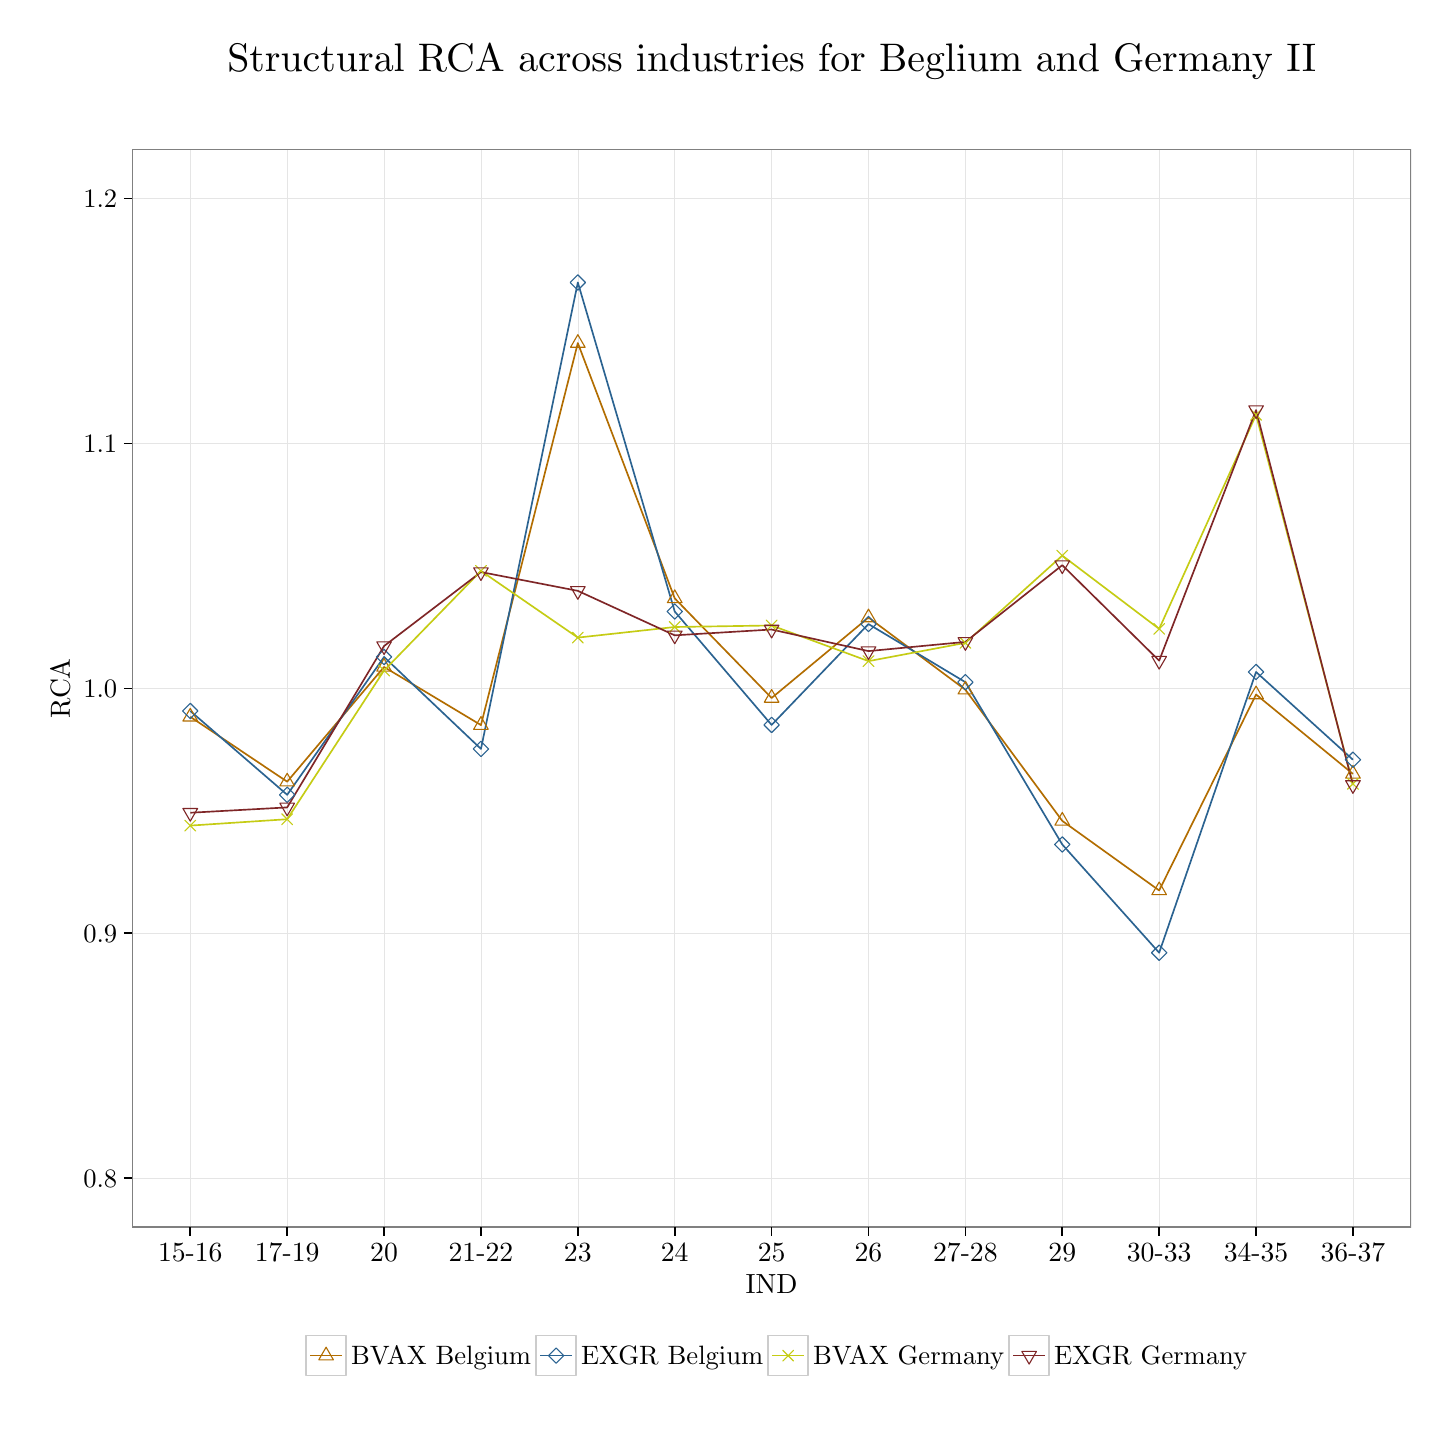
\begin{tikzpicture}[x=1pt,y=1pt]
\definecolor{fillColor}{RGB}{255,255,255}
\path[use as bounding box,fill=fillColor,fill opacity=0.00] (0,0) rectangle (505.89,505.89);
\begin{scope}
\path[clip] (  0.00,  0.00) rectangle (505.89,505.89);
\definecolor{drawColor}{RGB}{255,255,255}
\definecolor{fillColor}{RGB}{255,255,255}

\path[draw=drawColor,line width= 0.6pt,line join=round,line cap=round,fill=fillColor] (  0.00, -0.00) rectangle (505.89,505.89);
\end{scope}
\begin{scope}
\path[clip] ( 37.75, 72.44) rectangle (499.89,461.83);
\definecolor{fillColor}{RGB}{255,255,255}

\path[fill=fillColor] ( 37.75, 72.44) rectangle (499.89,461.83);
\definecolor{drawColor}{gray}{0.90}

\path[draw=drawColor,line width= 0.2pt,line join=round] ( 37.75, 90.14) --
	(499.89, 90.14);

\path[draw=drawColor,line width= 0.2pt,line join=round] ( 37.75,178.64) --
	(499.89,178.64);

\path[draw=drawColor,line width= 0.2pt,line join=round] ( 37.75,267.13) --
	(499.89,267.13);

\path[draw=drawColor,line width= 0.2pt,line join=round] ( 37.75,355.63) --
	(499.89,355.63);

\path[draw=drawColor,line width= 0.2pt,line join=round] ( 37.75,444.13) --
	(499.89,444.13);

\path[draw=drawColor,line width= 0.2pt,line join=round] ( 58.76, 72.44) --
	( 58.76,461.83);

\path[draw=drawColor,line width= 0.2pt,line join=round] ( 93.77, 72.44) --
	( 93.77,461.83);

\path[draw=drawColor,line width= 0.2pt,line join=round] (128.78, 72.44) --
	(128.78,461.83);

\path[draw=drawColor,line width= 0.2pt,line join=round] (163.79, 72.44) --
	(163.79,461.83);

\path[draw=drawColor,line width= 0.2pt,line join=round] (198.80, 72.44) --
	(198.80,461.83);

\path[draw=drawColor,line width= 0.2pt,line join=round] (233.81, 72.44) --
	(233.81,461.83);

\path[draw=drawColor,line width= 0.2pt,line join=round] (268.82, 72.44) --
	(268.82,461.83);

\path[draw=drawColor,line width= 0.2pt,line join=round] (303.83, 72.44) --
	(303.83,461.83);

\path[draw=drawColor,line width= 0.2pt,line join=round] (338.84, 72.44) --
	(338.84,461.83);

\path[draw=drawColor,line width= 0.2pt,line join=round] (373.85, 72.44) --
	(373.85,461.83);

\path[draw=drawColor,line width= 0.2pt,line join=round] (408.86, 72.44) --
	(408.86,461.83);

\path[draw=drawColor,line width= 0.2pt,line join=round] (443.87, 72.44) --
	(443.87,461.83);

\path[draw=drawColor,line width= 0.2pt,line join=round] (478.88, 72.44) --
	(478.88,461.83);
\definecolor{drawColor}{RGB}{178,109,0}

\path[draw=drawColor,line width= 0.6pt,line join=round] ( 58.76,256.88) --
	( 93.77,233.42) --
	(128.78,274.88) --
	(163.79,253.88) --
	(198.80,391.92) --
	(233.81,299.67) --
	(268.82,263.67) --
	(303.83,292.74) --
	(338.84,266.65) --
	(373.85,219.26) --
	(408.86,194.12) --
	(443.87,264.93) --
	(478.88,236.24);
\definecolor{drawColor}{RGB}{43,99,145}

\path[draw=drawColor,line width= 0.6pt,line join=round] ( 58.76,258.97) --
	( 93.77,228.68) --
	(128.78,278.49) --
	(163.79,245.26) --
	(198.80,413.81) --
	(233.81,294.92) --
	(268.82,253.93) --
	(303.83,290.39) --
	(338.84,269.38) --
	(373.85,210.73) --
	(408.86,171.61) --
	(443.87,273.07) --
	(478.88,241.36);
\definecolor{drawColor}{RGB}{197,204,20}

\path[draw=drawColor,line width= 0.6pt,line join=round] ( 58.76,217.56) --
	( 93.77,219.86) --
	(128.78,273.61) --
	(163.79,309.59) --
	(198.80,285.49) --
	(233.81,289.32) --
	(268.82,289.87) --
	(303.83,276.98) --
	(338.84,283.58) --
	(373.85,315.13) --
	(408.86,288.64) --
	(443.87,365.98) --
	(478.88,232.65);
\definecolor{drawColor}{RGB}{127,38,39}

\path[draw=drawColor,line width= 0.6pt,line join=round] ( 58.76,222.20) --
	( 93.77,224.13) --
	(128.78,282.44) --
	(163.79,309.18) --
	(198.80,302.38) --
	(233.81,286.31) --
	(268.82,288.41) --
	(303.83,280.61) --
	(338.84,283.93) --
	(373.85,311.66) --
	(408.86,277.15) --
	(443.87,367.71) --
	(478.88,232.26);
\definecolor{drawColor}{RGB}{178,109,0}

\path[draw=drawColor,line width= 0.4pt,line join=round,line cap=round] ( 58.76,259.93) --
	( 61.40,255.36) --
	( 56.11,255.36) --
	( 58.76,259.93);

\path[draw=drawColor,line width= 0.4pt,line join=round,line cap=round] ( 93.77,236.47) --
	( 96.41,231.89) --
	( 91.13,231.89) --
	( 93.77,236.47);

\path[draw=drawColor,line width= 0.4pt,line join=round,line cap=round] (128.78,277.93) --
	(131.42,273.36) --
	(126.14,273.36) --
	(128.78,277.93);

\path[draw=drawColor,line width= 0.4pt,line join=round,line cap=round] (163.79,256.93) --
	(166.43,252.35) --
	(161.15,252.35) --
	(163.79,256.93);

\path[draw=drawColor,line width= 0.4pt,line join=round,line cap=round] (198.80,394.97) --
	(201.44,390.39) --
	(196.16,390.39) --
	(198.80,394.97);

\path[draw=drawColor,line width= 0.4pt,line join=round,line cap=round] (233.81,302.72) --
	(236.45,298.14) --
	(231.17,298.14) --
	(233.81,302.72);

\path[draw=drawColor,line width= 0.4pt,line join=round,line cap=round] (268.82,266.72) --
	(271.46,262.14) --
	(266.18,262.14) --
	(268.82,266.72);

\path[draw=drawColor,line width= 0.4pt,line join=round,line cap=round] (303.83,295.79) --
	(306.47,291.22) --
	(301.19,291.22) --
	(303.83,295.79);

\path[draw=drawColor,line width= 0.4pt,line join=round,line cap=round] (338.84,269.70) --
	(341.48,265.13) --
	(336.20,265.13) --
	(338.84,269.70);

\path[draw=drawColor,line width= 0.4pt,line join=round,line cap=round] (373.85,222.31) --
	(376.49,217.74) --
	(371.21,217.74) --
	(373.85,222.31);

\path[draw=drawColor,line width= 0.4pt,line join=round,line cap=round] (408.86,197.17) --
	(411.51,192.59) --
	(406.22,192.59) --
	(408.86,197.17);

\path[draw=drawColor,line width= 0.4pt,line join=round,line cap=round] (443.87,267.98) --
	(446.52,263.41) --
	(441.23,263.41) --
	(443.87,267.98);

\path[draw=drawColor,line width= 0.4pt,line join=round,line cap=round] (478.88,239.29) --
	(481.53,234.71) --
	(476.24,234.71) --
	(478.88,239.29);
\definecolor{drawColor}{RGB}{197,204,20}

\path[draw=drawColor,line width= 0.4pt,line join=round,line cap=round] ( 56.80,215.59) -- ( 60.72,219.52);

\path[draw=drawColor,line width= 0.4pt,line join=round,line cap=round] ( 56.80,219.52) -- ( 60.72,215.59);

\path[draw=drawColor,line width= 0.4pt,line join=round,line cap=round] ( 91.81,217.90) -- ( 95.73,221.83);

\path[draw=drawColor,line width= 0.4pt,line join=round,line cap=round] ( 91.81,221.83) -- ( 95.73,217.90);

\path[draw=drawColor,line width= 0.4pt,line join=round,line cap=round] (126.82,271.65) -- (130.74,275.57);

\path[draw=drawColor,line width= 0.4pt,line join=round,line cap=round] (126.82,275.57) -- (130.74,271.65);

\path[draw=drawColor,line width= 0.4pt,line join=round,line cap=round] (161.83,307.63) -- (165.75,311.55);

\path[draw=drawColor,line width= 0.4pt,line join=round,line cap=round] (161.83,311.55) -- (165.75,307.63);

\path[draw=drawColor,line width= 0.4pt,line join=round,line cap=round] (196.84,283.52) -- (200.76,287.45);

\path[draw=drawColor,line width= 0.4pt,line join=round,line cap=round] (196.84,287.45) -- (200.76,283.52);

\path[draw=drawColor,line width= 0.4pt,line join=round,line cap=round] (231.85,287.36) -- (235.77,291.29);

\path[draw=drawColor,line width= 0.4pt,line join=round,line cap=round] (231.85,291.29) -- (235.77,287.36);

\path[draw=drawColor,line width= 0.4pt,line join=round,line cap=round] (266.86,287.91) -- (270.78,291.83);

\path[draw=drawColor,line width= 0.4pt,line join=round,line cap=round] (266.86,291.83) -- (270.78,287.91);

\path[draw=drawColor,line width= 0.4pt,line join=round,line cap=round] (301.87,275.02) -- (305.79,278.94);

\path[draw=drawColor,line width= 0.4pt,line join=round,line cap=round] (301.87,278.94) -- (305.79,275.02);

\path[draw=drawColor,line width= 0.4pt,line join=round,line cap=round] (336.88,281.61) -- (340.80,285.54);

\path[draw=drawColor,line width= 0.4pt,line join=round,line cap=round] (336.88,285.54) -- (340.80,281.61);

\path[draw=drawColor,line width= 0.4pt,line join=round,line cap=round] (371.89,313.16) -- (375.81,317.09);

\path[draw=drawColor,line width= 0.4pt,line join=round,line cap=round] (371.89,317.09) -- (375.81,313.16);

\path[draw=drawColor,line width= 0.4pt,line join=round,line cap=round] (406.90,286.68) -- (410.82,290.60);

\path[draw=drawColor,line width= 0.4pt,line join=round,line cap=round] (406.90,290.60) -- (410.82,286.68);

\path[draw=drawColor,line width= 0.4pt,line join=round,line cap=round] (441.91,364.02) -- (445.84,367.94);

\path[draw=drawColor,line width= 0.4pt,line join=round,line cap=round] (441.91,367.94) -- (445.84,364.02);

\path[draw=drawColor,line width= 0.4pt,line join=round,line cap=round] (476.92,230.69) -- (480.85,234.62);

\path[draw=drawColor,line width= 0.4pt,line join=round,line cap=round] (476.92,234.62) -- (480.85,230.69);
\definecolor{drawColor}{RGB}{43,99,145}

\path[draw=drawColor,line width= 0.4pt,line join=round,line cap=round] ( 55.98,258.97) --
	( 58.76,261.75) --
	( 61.53,258.97) --
	( 58.76,256.20) --
	( 55.98,258.97);

\path[draw=drawColor,line width= 0.4pt,line join=round,line cap=round] ( 90.99,228.68) --
	( 93.77,231.46) --
	( 96.54,228.68) --
	( 93.77,225.91) --
	( 90.99,228.68);

\path[draw=drawColor,line width= 0.4pt,line join=round,line cap=round] (126.00,278.49) --
	(128.78,281.26) --
	(131.55,278.49) --
	(128.78,275.71) --
	(126.00,278.49);

\path[draw=drawColor,line width= 0.4pt,line join=round,line cap=round] (161.01,245.26) --
	(163.79,248.04) --
	(166.56,245.26) --
	(163.79,242.49) --
	(161.01,245.26);

\path[draw=drawColor,line width= 0.4pt,line join=round,line cap=round] (196.02,413.81) --
	(198.80,416.58) --
	(201.57,413.81) --
	(198.80,411.03) --
	(196.02,413.81);

\path[draw=drawColor,line width= 0.4pt,line join=round,line cap=round] (231.04,294.92) --
	(233.81,297.69) --
	(236.58,294.92) --
	(233.81,292.14) --
	(231.04,294.92);

\path[draw=drawColor,line width= 0.4pt,line join=round,line cap=round] (266.05,253.93) --
	(268.82,256.71) --
	(271.60,253.93) --
	(268.82,251.16) --
	(266.05,253.93);

\path[draw=drawColor,line width= 0.4pt,line join=round,line cap=round] (301.06,290.39) --
	(303.83,293.17) --
	(306.61,290.39) --
	(303.83,287.62) --
	(301.06,290.39);

\path[draw=drawColor,line width= 0.4pt,line join=round,line cap=round] (336.07,269.38) --
	(338.84,272.16) --
	(341.62,269.38) --
	(338.84,266.61) --
	(336.07,269.38);

\path[draw=drawColor,line width= 0.4pt,line join=round,line cap=round] (371.08,210.73) --
	(373.85,213.51) --
	(376.63,210.73) --
	(373.85,207.96) --
	(371.08,210.73);

\path[draw=drawColor,line width= 0.4pt,line join=round,line cap=round] (406.09,171.61) --
	(408.86,174.39) --
	(411.64,171.61) --
	(408.86,168.84) --
	(406.09,171.61);

\path[draw=drawColor,line width= 0.4pt,line join=round,line cap=round] (441.10,273.07) --
	(443.87,275.85) --
	(446.65,273.07) --
	(443.87,270.30) --
	(441.10,273.07);

\path[draw=drawColor,line width= 0.4pt,line join=round,line cap=round] (476.11,241.36) --
	(478.88,244.14) --
	(481.66,241.36) --
	(478.88,238.59) --
	(476.11,241.36);
\definecolor{drawColor}{RGB}{127,38,39}

\path[draw=drawColor,line width= 0.4pt,line join=round,line cap=round] ( 58.76,219.15) --
	( 61.40,223.73) --
	( 56.11,223.73) --
	( 58.76,219.15);

\path[draw=drawColor,line width= 0.4pt,line join=round,line cap=round] ( 93.77,221.08) --
	( 96.41,225.66) --
	( 91.13,225.66) --
	( 93.77,221.08);

\path[draw=drawColor,line width= 0.4pt,line join=round,line cap=round] (128.78,279.39) --
	(131.42,283.97) --
	(126.14,283.97) --
	(128.78,279.39);

\path[draw=drawColor,line width= 0.4pt,line join=round,line cap=round] (163.79,306.13) --
	(166.43,310.70) --
	(161.15,310.70) --
	(163.79,306.13);

\path[draw=drawColor,line width= 0.4pt,line join=round,line cap=round] (198.80,299.33) --
	(201.44,303.91) --
	(196.16,303.91) --
	(198.80,299.33);

\path[draw=drawColor,line width= 0.4pt,line join=round,line cap=round] (233.81,283.26) --
	(236.45,287.83) --
	(231.17,287.83) --
	(233.81,283.26);

\path[draw=drawColor,line width= 0.4pt,line join=round,line cap=round] (268.82,285.36) --
	(271.46,289.94) --
	(266.18,289.94) --
	(268.82,285.36);

\path[draw=drawColor,line width= 0.4pt,line join=round,line cap=round] (303.83,277.56) --
	(306.47,282.14) --
	(301.19,282.14) --
	(303.83,277.56);

\path[draw=drawColor,line width= 0.4pt,line join=round,line cap=round] (338.84,280.88) --
	(341.48,285.46) --
	(336.20,285.46) --
	(338.84,280.88);

\path[draw=drawColor,line width= 0.4pt,line join=round,line cap=round] (373.85,308.61) --
	(376.49,313.19) --
	(371.21,313.19) --
	(373.85,308.61);

\path[draw=drawColor,line width= 0.4pt,line join=round,line cap=round] (408.86,274.10) --
	(411.51,278.68) --
	(406.22,278.68) --
	(408.86,274.10);

\path[draw=drawColor,line width= 0.4pt,line join=round,line cap=round] (443.87,364.66) --
	(446.52,369.24) --
	(441.23,369.24) --
	(443.87,364.66);

\path[draw=drawColor,line width= 0.4pt,line join=round,line cap=round] (478.88,229.21) --
	(481.53,233.78) --
	(476.24,233.78) --
	(478.88,229.21);
\definecolor{drawColor}{gray}{0.50}

\path[draw=drawColor,line width= 0.6pt,line join=round,line cap=round] ( 37.75, 72.44) rectangle (499.89,461.83);
\end{scope}
\begin{scope}
\path[clip] (  0.00,  0.00) rectangle (505.89,505.89);
\definecolor{drawColor}{RGB}{0,0,0}

\node[text=drawColor,anchor=base east,inner sep=0pt, outer sep=0pt, scale=  0.96] at ( 32.35, 86.83) {0.8};

\node[text=drawColor,anchor=base east,inner sep=0pt, outer sep=0pt, scale=  0.96] at ( 32.35,175.33) {0.9};

\node[text=drawColor,anchor=base east,inner sep=0pt, outer sep=0pt, scale=  0.96] at ( 32.35,263.83) {1.0};

\node[text=drawColor,anchor=base east,inner sep=0pt, outer sep=0pt, scale=  0.96] at ( 32.35,352.33) {1.1};

\node[text=drawColor,anchor=base east,inner sep=0pt, outer sep=0pt, scale=  0.96] at ( 32.35,440.83) {1.2};
\end{scope}
\begin{scope}
\path[clip] (  0.00,  0.00) rectangle (505.89,505.89);
\definecolor{drawColor}{RGB}{0,0,0}

\path[draw=drawColor,line width= 0.6pt,line join=round] ( 34.75, 90.14) --
	( 37.75, 90.14);

\path[draw=drawColor,line width= 0.6pt,line join=round] ( 34.75,178.64) --
	( 37.75,178.64);

\path[draw=drawColor,line width= 0.6pt,line join=round] ( 34.75,267.13) --
	( 37.75,267.13);

\path[draw=drawColor,line width= 0.6pt,line join=round] ( 34.75,355.63) --
	( 37.75,355.63);

\path[draw=drawColor,line width= 0.6pt,line join=round] ( 34.75,444.13) --
	( 37.75,444.13);
\end{scope}
\begin{scope}
\path[clip] (  0.00,  0.00) rectangle (505.89,505.89);
\definecolor{drawColor}{RGB}{0,0,0}

\path[draw=drawColor,line width= 0.6pt,line join=round] ( 58.76, 69.44) --
	( 58.76, 72.44);

\path[draw=drawColor,line width= 0.6pt,line join=round] ( 93.77, 69.44) --
	( 93.77, 72.44);

\path[draw=drawColor,line width= 0.6pt,line join=round] (128.78, 69.44) --
	(128.78, 72.44);

\path[draw=drawColor,line width= 0.6pt,line join=round] (163.79, 69.44) --
	(163.79, 72.44);

\path[draw=drawColor,line width= 0.6pt,line join=round] (198.80, 69.44) --
	(198.80, 72.44);

\path[draw=drawColor,line width= 0.6pt,line join=round] (233.81, 69.44) --
	(233.81, 72.44);

\path[draw=drawColor,line width= 0.6pt,line join=round] (268.82, 69.44) --
	(268.82, 72.44);

\path[draw=drawColor,line width= 0.6pt,line join=round] (303.83, 69.44) --
	(303.83, 72.44);

\path[draw=drawColor,line width= 0.6pt,line join=round] (338.84, 69.44) --
	(338.84, 72.44);

\path[draw=drawColor,line width= 0.6pt,line join=round] (373.85, 69.44) --
	(373.85, 72.44);

\path[draw=drawColor,line width= 0.6pt,line join=round] (408.86, 69.44) --
	(408.86, 72.44);

\path[draw=drawColor,line width= 0.6pt,line join=round] (443.87, 69.44) --
	(443.87, 72.44);

\path[draw=drawColor,line width= 0.6pt,line join=round] (478.88, 69.44) --
	(478.88, 72.44);
\end{scope}
\begin{scope}
\path[clip] (  0.00,  0.00) rectangle (505.89,505.89);
\definecolor{drawColor}{RGB}{0,0,0}

\node[text=drawColor,anchor=base,inner sep=0pt, outer sep=0pt, scale=  1.00] at ( 58.76, 60.15) {15-16};

\node[text=drawColor,anchor=base,inner sep=0pt, outer sep=0pt, scale=  1.00] at ( 93.77, 60.15) {17-19};

\node[text=drawColor,anchor=base,inner sep=0pt, outer sep=0pt, scale=  1.00] at (128.78, 60.15) {20};

\node[text=drawColor,anchor=base,inner sep=0pt, outer sep=0pt, scale=  1.00] at (163.79, 60.15) {21-22};

\node[text=drawColor,anchor=base,inner sep=0pt, outer sep=0pt, scale=  1.00] at (198.80, 60.15) {23};

\node[text=drawColor,anchor=base,inner sep=0pt, outer sep=0pt, scale=  1.00] at (233.81, 60.15) {24};

\node[text=drawColor,anchor=base,inner sep=0pt, outer sep=0pt, scale=  1.00] at (268.82, 60.15) {25};

\node[text=drawColor,anchor=base,inner sep=0pt, outer sep=0pt, scale=  1.00] at (303.83, 60.15) {26};

\node[text=drawColor,anchor=base,inner sep=0pt, outer sep=0pt, scale=  1.00] at (338.84, 60.15) {27-28};

\node[text=drawColor,anchor=base,inner sep=0pt, outer sep=0pt, scale=  1.00] at (373.85, 60.15) {29};

\node[text=drawColor,anchor=base,inner sep=0pt, outer sep=0pt, scale=  1.00] at (408.86, 60.15) {30-33};

\node[text=drawColor,anchor=base,inner sep=0pt, outer sep=0pt, scale=  1.00] at (443.87, 60.15) {34-35};

\node[text=drawColor,anchor=base,inner sep=0pt, outer sep=0pt, scale=  1.00] at (478.88, 60.15) {36-37};
\end{scope}
\begin{scope}
\path[clip] (  0.00,  0.00) rectangle (505.89,505.89);
\definecolor{drawColor}{RGB}{0,0,0}

\node[text=drawColor,anchor=base,inner sep=0pt, outer sep=0pt, scale=  1.00] at (268.82, 48.46) {IND};
\end{scope}
\begin{scope}
\path[clip] (  0.00,  0.00) rectangle (505.89,505.89);
\definecolor{drawColor}{RGB}{0,0,0}

\node[text=drawColor,rotate= 90.00,anchor=base,inner sep=0pt, outer sep=0pt, scale=  1.00] at ( 15.29,267.13) {RCA};
\end{scope}
\begin{scope}
\path[clip] (  0.00,  0.00) rectangle (505.89,505.89);
\definecolor{fillColor}{RGB}{255,255,255}

\path[fill=fillColor] ( 92.72, 14.54) rectangle (444.92, 37.53);
\end{scope}
\begin{scope}
\path[clip] (  0.00,  0.00) rectangle (505.89,505.89);
\definecolor{drawColor}{gray}{0.80}
\definecolor{fillColor}{RGB}{255,255,255}

\path[draw=drawColor,line width= 0.6pt,line join=round,line cap=round,fill=fillColor] (100.60, 18.80) rectangle (115.05, 33.26);
\end{scope}
\begin{scope}
\path[clip] (  0.00,  0.00) rectangle (505.89,505.89);
\definecolor{drawColor}{RGB}{178,109,0}

\path[draw=drawColor,line width= 0.6pt,line join=round] (102.05, 26.03) -- (113.61, 26.03);
\end{scope}
\begin{scope}
\path[clip] (  0.00,  0.00) rectangle (505.89,505.89);
\definecolor{drawColor}{RGB}{178,109,0}

\path[draw=drawColor,line width= 0.4pt,line join=round,line cap=round] (107.83, 29.08) --
	(110.47, 24.51) --
	(105.19, 24.51) --
	(107.83, 29.08);
\end{scope}
\begin{scope}
\path[clip] (  0.00,  0.00) rectangle (505.89,505.89);
\definecolor{drawColor}{gray}{0.80}
\definecolor{fillColor}{RGB}{255,255,255}

\path[draw=drawColor,line width= 0.6pt,line join=round,line cap=round,fill=fillColor] (183.72, 18.80) rectangle (198.17, 33.26);
\end{scope}
\begin{scope}
\path[clip] (  0.00,  0.00) rectangle (505.89,505.89);
\definecolor{drawColor}{RGB}{43,99,145}

\path[draw=drawColor,line width= 0.6pt,line join=round] (185.17, 26.03) -- (196.73, 26.03);
\end{scope}
\begin{scope}
\path[clip] (  0.00,  0.00) rectangle (505.89,505.89);
\definecolor{drawColor}{RGB}{43,99,145}

\path[draw=drawColor,line width= 0.4pt,line join=round,line cap=round] (188.17, 26.03) --
	(190.95, 28.81) --
	(193.72, 26.03) --
	(190.95, 23.26) --
	(188.17, 26.03);
\end{scope}
\begin{scope}
\path[clip] (  0.00,  0.00) rectangle (505.89,505.89);
\definecolor{drawColor}{gray}{0.80}
\definecolor{fillColor}{RGB}{255,255,255}

\path[draw=drawColor,line width= 0.6pt,line join=round,line cap=round,fill=fillColor] (267.57, 18.80) rectangle (282.03, 33.26);
\end{scope}
\begin{scope}
\path[clip] (  0.00,  0.00) rectangle (505.89,505.89);
\definecolor{drawColor}{RGB}{197,204,20}

\path[draw=drawColor,line width= 0.6pt,line join=round] (269.02, 26.03) -- (280.58, 26.03);
\end{scope}
\begin{scope}
\path[clip] (  0.00,  0.00) rectangle (505.89,505.89);
\definecolor{drawColor}{RGB}{197,204,20}

\path[draw=drawColor,line width= 0.4pt,line join=round,line cap=round] (272.84, 24.07) -- (276.76, 27.99);

\path[draw=drawColor,line width= 0.4pt,line join=round,line cap=round] (272.84, 27.99) -- (276.76, 24.07);
\end{scope}
\begin{scope}
\path[clip] (  0.00,  0.00) rectangle (505.89,505.89);
\definecolor{drawColor}{gray}{0.80}
\definecolor{fillColor}{RGB}{255,255,255}

\path[draw=drawColor,line width= 0.6pt,line join=round,line cap=round,fill=fillColor] (354.65, 18.80) rectangle (369.10, 33.26);
\end{scope}
\begin{scope}
\path[clip] (  0.00,  0.00) rectangle (505.89,505.89);
\definecolor{drawColor}{RGB}{127,38,39}

\path[draw=drawColor,line width= 0.6pt,line join=round] (356.09, 26.03) -- (367.66, 26.03);
\end{scope}
\begin{scope}
\path[clip] (  0.00,  0.00) rectangle (505.89,505.89);
\definecolor{drawColor}{RGB}{127,38,39}

\path[draw=drawColor,line width= 0.4pt,line join=round,line cap=round] (361.88, 22.98) --
	(364.52, 27.56) --
	(359.23, 27.56) --
	(361.88, 22.98);
\end{scope}
\begin{scope}
\path[clip] (  0.00,  0.00) rectangle (505.89,505.89);
\definecolor{drawColor}{RGB}{0,0,0}

\node[text=drawColor,anchor=base west,inner sep=0pt, outer sep=0pt, scale=  0.96] at (116.86, 22.72) {BVAX Belgium};
\end{scope}
\begin{scope}
\path[clip] (  0.00,  0.00) rectangle (505.89,505.89);
\definecolor{drawColor}{RGB}{0,0,0}

\node[text=drawColor,anchor=base west,inner sep=0pt, outer sep=0pt, scale=  0.96] at (199.98, 22.72) {EXGR Belgium};
\end{scope}
\begin{scope}
\path[clip] (  0.00,  0.00) rectangle (505.89,505.89);
\definecolor{drawColor}{RGB}{0,0,0}

\node[text=drawColor,anchor=base west,inner sep=0pt, outer sep=0pt, scale=  0.96] at (283.83, 22.72) {BVAX Germany};
\end{scope}
\begin{scope}
\path[clip] (  0.00,  0.00) rectangle (505.89,505.89);
\definecolor{drawColor}{RGB}{0,0,0}

\node[text=drawColor,anchor=base west,inner sep=0pt, outer sep=0pt, scale=  0.96] at (370.91, 22.72) {EXGR Germany};
\end{scope}
\begin{scope}
\path[clip] (  0.00,  0.00) rectangle (505.89,505.89);
\definecolor{drawColor}{RGB}{0,0,0}

\node[text=drawColor,anchor=base west,inner sep=0pt, outer sep=0pt, scale=  1.44] at ( 72.14,489.97) {Structural RCA across industries for Beglium and Germany II};
\end{scope}
\end{tikzpicture}
